%\vspace*{-0.4cm}
\chapter[Thème 2 $-$ Limites de fonctions]{Thème 2 : Modèles continus \\Limites de fonctions}
\thispagestyle{fancy}

\vspace*{-0.6cm}
\section{Limite d'une fonction à l'infini}
\subsection{Limite infinie en $\infty$}
\section*{Définition :}
\begin{bdefi}
	\phantom{$\dfrac{1}{2}$}\pointilles[\textwidth-0.2cm]
	
	\phantom{$\dfrac{1}{2}$}\pointilles[\textwidth-0.2cm]
\end{bdefi}
\begin{brmq}
	On a une définition analogue en $-\infty$.
\end{brmq}

\begin{bexemple}

\begin{minipage}[c]{0.58\linewidth}
La fonction définie par $f(x)=x^{2}$ a pour limite $+\infty$ lorsque $x$ tend vers $+\infty$.\\
On a par exemple : $f(100)=100^{2}=10000$
	
\quad \quad \quad \quad \quad \quad \quad \quad$f(1000)=1000^{2}=1000000$

Les valeurs de la fonction deviennent aussi grandes que l'on veut dès que $x$ est suffisamment grand.\\
\end{minipage} \hfill
\begin{minipage}[c]{0.38\linewidth}
	
\includegraphics[scale=0.22]{T05-Crs-Img01}	
\end{minipage}	
\end{bexemple}

\begin{brmqs}
	\begin{itemRem}
		\item Une fonction qui tend vers $+\infty$ lorsque $x$ tend vers $+\infty$ n'est pas nécessairement croissante. Par exemple :
		\begin{center}
				
\includegraphics[scale=0.2]{T05-Crs-Img02}
		\end{center}
		\item Il existe des fonctions qui ne possèdent pas de limite infinie. C'est le cas des fonctions sinusoïdales.
		\begin{center}
			
\includegraphics[scale=0.2]{T05-Crs-Img03}
		\end{center}
		
	\end{itemRem}
\end{brmqs}


\subsection{Limite finie en $\infty$}
\begin{bdefi}
	\phantom{$\dfrac{1}{2}$}\pointilles[\textwidth-0.2cm]
	
	\phantom{$\dfrac{1}{2}$}\pointilles[\textwidth-0.2cm]
	
	\phantom{$\dfrac{1}{2}$}\pointilles[\textwidth-0.2cm]
\end{bdefi}
\begin{brmq}
	On a une définition analogue en $-\infty$.
\end{brmq}

\begin{bexemple}
	
	\begin{minipage}[c]{0.28\linewidth}
		La fonction définie par $f(x)=2+\dfrac{1}{x}$ a pour limite 2 lorsque $x$ tend vers $+\infty$. On a par exemple :
		
		$$
		\begin{aligned}
			& f(100)=2+\frac{1}{100}=2,01 \\
			& \begin{aligned}
				f(10000) & =2+\frac{1}{10000} \\
				& =2,0001
			\end{aligned}
		\end{aligned}
		$$
	\end{minipage} \hfill
	\begin{minipage}[c]{0.68\linewidth}
		
\includegraphics[scale=0.3]{T05-Crs-Img04}
	\end{minipage}
	Les valeurs de la fonction se resserrent autour de 2 dès que $x$ est suffisamment grand. La courbe de la fonction "se rapproche" de la droite d'équation $y=2$ sans jamais la toucher.	
\end{bexemple}

\begin{bdefi}
\phantom{$\dfrac{1}{2}$}\pointilles[\textwidth-0.2cm]

\phantom{$\dfrac{1}{2}$}\pointilles[\textwidth-0.2cm]
\begin{center}
	
\includegraphics[scale=0.25]{T05-Crs-Img05}
\end{center}

\end{bdefi}

\begin{brmqs}
	\begin{itemRem}
		\item Lorsque $x$ tend vers $+\infty$, la courbe de la fonction "se rapproche" de son asymptote.
		\item On a une définition analogue en $-\infty$.
	\end{itemRem}
\end{brmqs}



\subsection{Limites des fonctions de référence}

\begin{bprops}
	\begin{itemProp}
		\item \phantom{$\dfrac{1}{2}$}\pointilles[\textwidth-0.8cm]
		\item \phantom{$\dfrac{1}{2}$}\pointilles[\textwidth-0.8cm]
		\item \phantom{$\dfrac{1}{2}$}\pointilles[\textwidth-0.8cm]
		\item \phantom{$\dfrac{1}{2}$}\pointilles[\textwidth-0.8cm]
		\item \phantom{$\dfrac{1}{2}$}\pointilles[\textwidth-0.8cm]
	\end{itemProp}
\end{bprops}

\section{Limite d'une fonction en un réel A}
\subsection{Définition}
\begin{bdefi}
\phantom{$\dfrac{1}{2}$}\pointilles[\textwidth-0.2cm]

\phantom{$\dfrac{1}{2}$}\pointilles[\textwidth-0.2cm]

\phantom{$\dfrac{1}{2}$}\pointilles[\textwidth-0.2cm]
\end{bdefi}

\begin{bexemple}
	
	\begin{minipage}[c]{0.53\linewidth}
		La fonction définie par $f(x)=\dfrac{1}{3-x}+1$ a pour limite $+\infty$ lorsque $x$ tend vers 3 .\\
		On a par exemple :\\
		$f(2,99)=\dfrac{1}{3-2,99}+1=101$\\
		$f(2,9999)=\dfrac{1}{3-2,9999}+1=10001$
		
		Les valeurs de la fonction deviennent aussi grandes que l'on veut dès que $x$ est suffisamment proche de 3 .
		
		La courbe de la fonction "se rapproche" de la droite d'équation $x=3$ sans jamais la toucher.\\
	\end{minipage} \hfill
	\begin{minipage}[c]{0.45\linewidth}
		
\includegraphics[scale=0.25]{T05-Crs-Img06}
	\end{minipage}	
\end{bexemple}

\begin{bdefi}
	\phantom{$\dfrac{1}{2}$}\pointilles[\textwidth-0.8cm]
	
	\phantom{$\dfrac{1}{2}$}\pointilles[\textwidth-0.8cm]
	\begin{center}
		
\includegraphics[scale=0.24]{T05-Crs-Img07}
	\end{center}
	
\end{bdefi}

\subsection{Limite à gauche, limite à droite}

\begin{bexemple}
	
	\begin{minipage}[c]{0.53\linewidth}
		Considérons la fonction inverse définie sur $\mathbb{R}^{*}$ par $f(x)=\frac{1}{x}$.\\
		La fonction $f$ admet des limites différentes en 0 selon que :\\
		$x>0$ ou $x<0$.
		
		\begin{itemEx}
			\item Si $x>0$ : Lorsque $x$ tend vers 0, $f(x)$ tend vers $+\infty$ et on note:\\
			$\lim _{\substack{x \rightarrow 0 \\ x>0}} f(x)=+\infty$ ou $\lim _{x \rightarrow 0^{+}} f(x)=+\infty$.\\
			On parle de limite à droite de 0
			\item Si $x<0$ : Lorsque $x$ tend vers 0, $f(x)$ tend vers $-\infty$ et on note:\\
			$\lim _{\substack{x \rightarrow 0 \\ x<0}} f(x)=-\infty$ ou $\lim _{x \rightarrow 0^{-}} f(x)=-\infty$.\\
			On parle de limite à gauche de $\mathbf{0}$.\\
			
		\end{itemEx}
	\end{minipage} \hfill
	\begin{minipage}[c]{0.45\linewidth}
		
\includegraphics[scale=0.23]{T05-Crs-Img08}
	\end{minipage}	
\end{bexemple}

\begin{bmethodet}{Déterminer graphiquement des limites d'une fonction}
	\grasInMet{Enoncé:}
	
	On donne ci-dessous la représentation graphique de la fonction $f$.
	\begin{enumMet}
		\item Lire graphiquement les limites en $-\infty$, en $+\infty$, en -4 et en 5 .
		\item Compléter alors le tableau de variations de $f$.
		\begin{center}
			\begin{tikzpicture}
				\tkzTabInit{$x$ / 1 , $f(x)$ / 1.5}{$-\infty$, $-4$, $2$, 5, $+\infty$}
				\tkzTabVar{}
			\end{tikzpicture}
		\end{center}
		\begin{center}
			
\includegraphics[scale=0.25]{T05-Crs-Img09}
		\end{center}
	\end{enumMet}
	\ \\
	\grasInMet{Solution}
		\begin{center}
			
\includegraphics[scale=0.25]{T05-Crs-Img10}
		\end{center}
\end{bmethodet}

\section{Opérations sur les limites}

\subsection{Utiliser les propriétés des opérations sur les limites}

$\alpha$ peut désigner $+\infty,-\infty$ ou un nombre réel.


\subsection*{SOMME}
\begin{center}
	\begin{tabular}{|l|c|c|c|c|c|c|}
		\hline
		$\lim \limits_{x \rightarrow \alpha} f(x)=$ & $L$ & $L$ & $L$ & $+\infty$ & $-\infty$ & $+\infty$ \\
		\hline
		$\lim \limits_{x \rightarrow \alpha} g(x)=$ & $L^{\prime}$ & $+\infty$ & $-\infty$ & $+\infty$ & $-\infty$ & $-\infty$ \\
		\hline
		$\lim \limits_{x \rightarrow \alpha} f(x)+g(x)=$ & $L+L^{\prime}$ & $+\infty$ & $-\infty$ & $+\infty$ & $-\infty$ & F.I.* \\
		\hline
	\end{tabular}
\end{center}

	* Forme indéterminée: On ne peut pas prévoir la limite éventuelle.

\subsection*{PRODUIT}

\begin{center}
	\begin{tabular}{|l|c|c|c|c|}
		\hline
		$\lim \limits_{x \rightarrow \alpha} f(x)=$ & $L$ & $L$ & $\infty$ & 0 \\
		\hline
		$\lim \limits_{x \rightarrow \alpha} g(x)=$ & $L^{\prime}$ & $\infty$ & $\infty$ & $\infty$ \\
		\hline
		$\lim \limits_{x \rightarrow \alpha} f(x) \times g(x)=$ & $L \times L^{\prime}$ & $\infty$ & $\infty$ & F.I. \\
		\hline
	\end{tabular}
\end{center}

On applique la règle des signes pour déterminer si le produit est $+\infty$ ou $-\infty$.

\subsection*{QUOTIENT}

\begin{center}
	\begin{tabular}{|c|c|c|c|c|c|c|}
		\hline
		$\lim \limits_{x \rightarrow \alpha} f(x)=$ & $L$ & $L \neq 0$ & $L$ & $\infty$ & $\infty$ & 0 \\
		\hline
		$\lim \limits_{x \rightarrow \alpha} g(x)=$ & $L^{\prime} \neq 0$ & 0 & $\infty$ & $L$ & $\infty$ & 0 \\
		\hline
		$\lim \limits_{x \rightarrow \alpha} \dfrac{f(x)}{g(x)}=$ & $\dfrac{L}{L^{\prime}}$ & $\infty$ & 0 & $\infty$ & F.I. & F.I. \\
		\hline
	\end{tabular}
\end{center}

On applique la règle des signes pour déterminer si le quotient est $+\infty$ ou $-\infty$.

\begin{bmethodet}{Calculer la limite d'une fonction à l'aide des formules d'opération}
	\grasInMet{Enoncé:}
	
	Déterminer les limites suivantes :
	\begin{enumMet}
		\item $\lim \limits_{x \rightarrow-\infty}(x-5)\left(3+x^{2}\right)$
		\item $\lim \limits_{x \rightarrow 3^{-}} \dfrac{1-2 x}{x-3}$
	\end{enumMet}
\end{bmethodet}

\begin{bmethodet}{Déterminer une asymptote}
	\grasInMet{Enoncé:}
	
	Soit $f$ la fonction définie sur $\mathbb{R} \backslash\{1\}$ par $f(x)=\dfrac{-2}{1-x}$.\\
	Démontrer que la courbe représentative de la fonction $f$ admet des asymptotes dont on précisera la nature et les équations.
	
	\ \\
	\grasInMet{Solution}
	\begin{center}
		
\includegraphics[scale=0.25]{T05-Crs-Img11}
	\end{center}
	
\end{bmethodet}

\section{Calculs de limites par composition et comparaison}
\subsection{Composition de limites}

\begin{bmethodet}{Déterminer la limite d'une fonction composée}
	\grasInMet{Enoncé:}
	
	Soit la fonction $f$ définie sur $\left[\dfrac{1}{2} ;+\infty\left[\operatorname{par}: f(x)=\sqrt{2-\frac{1}{x}}\right.\right.$\\
	Calculer la limite de la fonction $f$ en $+\infty$.
	

\end{bmethodet}

\subsection{Comparaison}

\begin{bmethodet}{Calculer une limite par comparaison}
	\grasInMet{Enoncé:}
	
	Calculer : $\lim \limits_{x \rightarrow+\infty} x+\sin x$
\end{bmethodet}